\section{Implementacja}
\label{chapter:3}
\subsection{Wymagania funkcjonalne}
Użytkownik może:
\begin{itemize}
    \item podać ścieżkę do pliku będącego przeszukiwanym tekstem,
    \item podać przeszukiwany tekst w postaci ciągu znaków (parametr wywołania programu),
    \item podać szukany wzorzec,
    \item zobaczyć wystąpienia (lub ich brak) wzorca w tekście,
    \item przeprowadzić testy wydajności implementacji algorytmu dla danego pliku i danych wzorców.
\end{itemize}
\subsection{Wymagania niefunkcjonalne}
Implementowany program:
\begin{itemize}
    \item wykorzystuje technologię \textbf{NVIDIA CUDA},
    \item wykorzystuje narzędzie \textbf{CMake} do procesu kompilacji,
    \item pisany jest w języku programowania \textbf{C++20},
    \item korzysta z kompilatorów: \textbf{gcc} oraz \textbf{cygwin}
\end{itemize}

\newpage
\subsection{Architektura}
Ze względu na złożoność problemu, program został podzielony na mniejsze, niezależne moduły:
\begin{itemize}
    \item moduł odpowiedzialny za wczytywanie tekstu,
    \item moduł odpowiedzialny za dzielenie tekstu na mniejsze fragmenty,
    \item moduł obliczający wartości haszów,
    \item moduł odpowiedzialny za przeprowadzanie pomiarów wydajności działania programu,
    \item moduł główny, zarządzający działaniem całego programu.
\end{itemize}
Podział na moduły został zaprezentowany na rysunku \ref{fig:dir_structure}.
\begin{figure}[H]
    \centering
    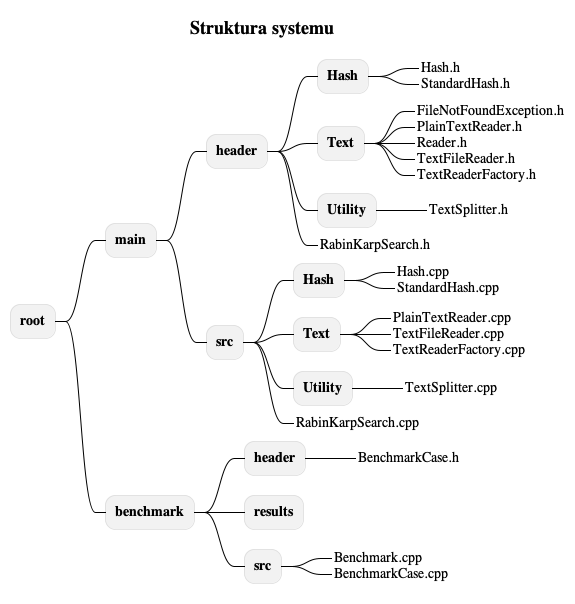
\includegraphics[scale=0.65]{images/uml/DirStructure.png}
    \caption{Struktura projektowanego systemu}
    \label{fig:dir_structure}
\end{figure}
Pomiędzy wymienionymi modułami występują zależności przedstawione na rysnku \ref{fig:rabin_karp_search}.
\begin{figure}[H]
    \centering
    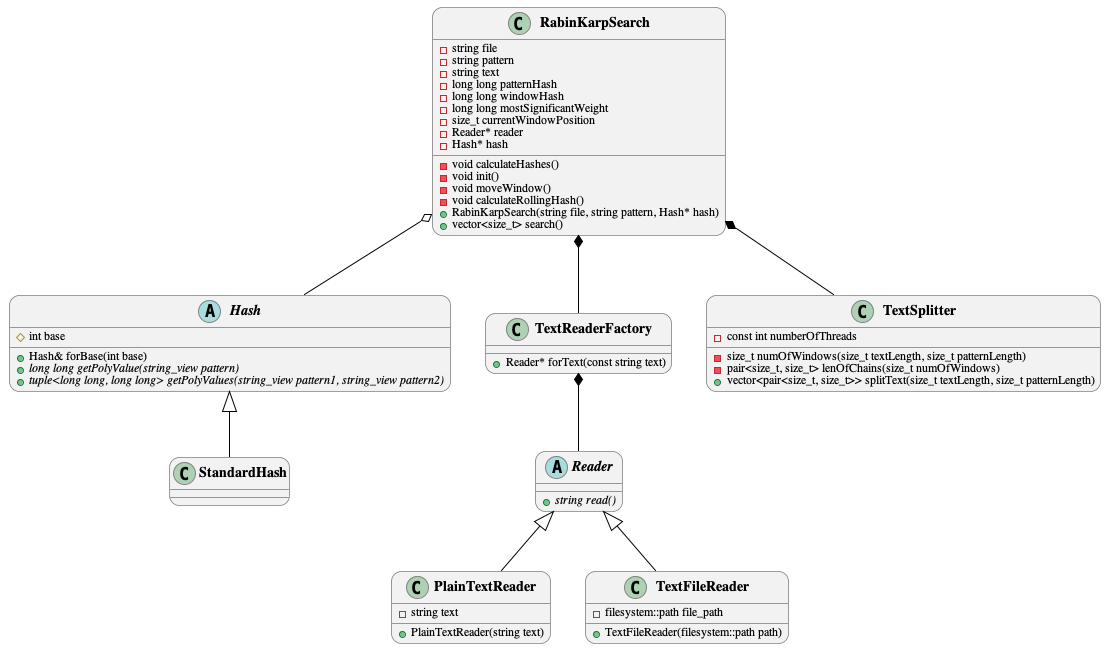
\includegraphics[width=\linewidth]{images/uml/RabinKarpSearch.png}
    \caption{Zależności pomiędzy modułami programu}
    \label{fig:rabin_karp_search}
\end{figure}
Na listingu \ref{lst:main_cpu} zaprezentowano przykładowe użycie modułu \textit{RabinKarpSearch} w wersji \textbf{CPU}. 
\begin{lstinputlisting}[language=C++, label=lst:main_cpu, caption=Przykładowe użycie modułu \textit{RabinKarpSearch} w wersji \textbf{CPU}]{listings/main_cpu.tex}
\end{lstinputlisting}

\subsection{Sposób równoleglenia operacji}
\label{subsec:parallelism}
Głównym aspektem równoleglenia implementacji algorytmu \textit{Rabina-Karpa} jest podział tekstu na zazębiające się podzbiory przeszukiwanego tekstu. W tym kontekście \textit{zazębiające się} oznacza, że wątki \textbf{GPU} analizują niezależnie od siebie i w niekontrolowanej kolejności określone podzbiory przeszukiwanego tekstu, symulując działanie \textit{x} niezależnych, sekwencyjnych instancji przeszukujących odpowiednio mniejszy fragment tekstu, który \say{nachodzi} na sąsiedni fragment tekstu. Sumarycznie, te \textit{x} sekwencyjnych instancji przeszukuje cały, zadany przez użytkownika, tekst. Proces podziału, na opisane fragmenty, został konceptualnie przedstawiony na rysunku \ref{fig:text_splitting}.
\begin{figure}[H]
    \centering
    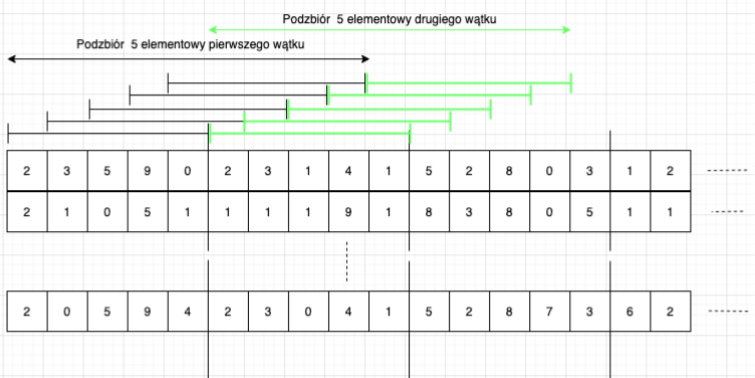
\includegraphics[width=\linewidth]{images/TextSplitting.png}
    \caption{Podział tekstu na zazębiające się fragmenty}
    \label{fig:text_splitting}
\end{figure}
Wiedząc, jak działa dzielenie tekstu, należy wydobyć taką liczbę fragmentów tekstu oraz dostosować długość pojedynczego fragmentu tak, aby każdy z wątków był równomierne obciążony i mógł przetworzyć możliwie jak największe fragmenty tekstu. Do tego celu proponujemy następujące rozwiązanie. 
\newpage
Niech dane będą: \textit{L} - długość przeszukiwanego tekstu, \textit{T} - liczba wątków, \textit{S} - długość szukanego wzorca, wtedy \textit{$C_i$} - długość fragmentu tekstu dla \textit{i-tego} wątku można określić zależnością:
\[
C_{i} = \begin{cases}
    \frac{L-S}{T} + 1& \text{dla i < (L - S) mod T}, \\
    \frac{L-S}{T}& \text{dla i $\geq$ (L - S) mod T}
\end{cases}
\]
Proces wykonywania się algorytmu z wykorzystaniem \textbf{GPU} został przedstawiony na rysnku \ref{fig:flow_chart}.
\begin{figure}[H]
    \centering
    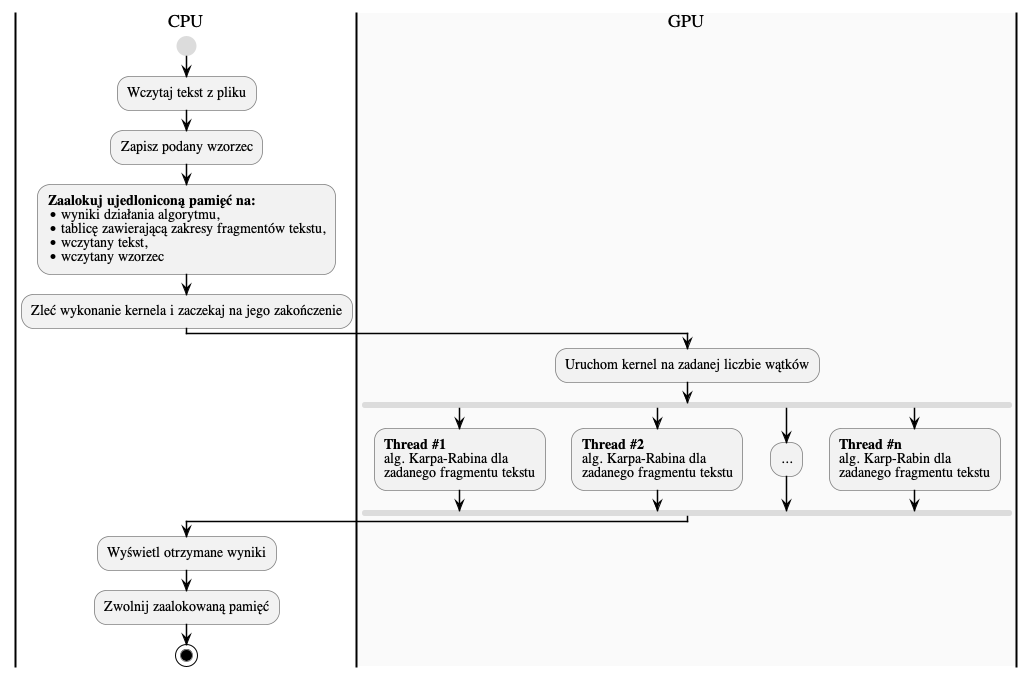
\includegraphics[width=\linewidth]{images/uml/FlowChart.png}
    \caption{Schemat działania programu dla wersji \textbf{GPU}}
    \label{fig:flow_chart}
\end{figure}

\newpage
Natomiast na listingu \ref{lst:main_gpu} przedstawiono przykładowe użycie modułu \textit{RabinKarpSearch} w wersji \textbf{GPU}.
\begin{lstinputlisting}[language=C++, label=lst:main_gpu, caption=Przykładowe użycie modułu \textit{RabinKarpSearch} w wersji \textbf{GPU}]{listings/main_gpu.tex}
\end{lstinputlisting}